\documentclass[runningheads]{llncs}\usepackage[]{graphicx}\usepackage[]{color}
% maxwidth is the original width if it is less than linewidth
% otherwise use linewidth (to make sure the graphics do not exceed the margin)
\makeatletter
\def\maxwidth{ %
  \ifdim\Gin@nat@width>\linewidth
    \linewidth
  \else
    \Gin@nat@width
  \fi
}
\makeatother

\definecolor{fgcolor}{rgb}{0.345, 0.345, 0.345}
\newcommand{\hlnum}[1]{\textcolor[rgb]{0.686,0.059,0.569}{#1}}%
\newcommand{\hlstr}[1]{\textcolor[rgb]{0.192,0.494,0.8}{#1}}%
\newcommand{\hlcom}[1]{\textcolor[rgb]{0.678,0.584,0.686}{\textit{#1}}}%
\newcommand{\hlopt}[1]{\textcolor[rgb]{0,0,0}{#1}}%
\newcommand{\hlstd}[1]{\textcolor[rgb]{0.345,0.345,0.345}{#1}}%
\newcommand{\hlkwa}[1]{\textcolor[rgb]{0.161,0.373,0.58}{\textbf{#1}}}%
\newcommand{\hlkwb}[1]{\textcolor[rgb]{0.69,0.353,0.396}{#1}}%
\newcommand{\hlkwc}[1]{\textcolor[rgb]{0.333,0.667,0.333}{#1}}%
\newcommand{\hlkwd}[1]{\textcolor[rgb]{0.737,0.353,0.396}{\textbf{#1}}}%
\let\hlipl\hlkwb

\usepackage{framed}
\makeatletter
\newenvironment{kframe}{%
 \def\at@end@of@kframe{}%
 \ifinner\ifhmode%
  \def\at@end@of@kframe{\end{minipage}}%
  \begin{minipage}{\columnwidth}%
 \fi\fi%
 \def\FrameCommand##1{\hskip\@totalleftmargin \hskip-\fboxsep
 \colorbox{shadecolor}{##1}\hskip-\fboxsep
     % There is no \\@totalrightmargin, so:
     \hskip-\linewidth \hskip-\@totalleftmargin \hskip\columnwidth}%
 \MakeFramed {\advance\hsize-\width
   \@totalleftmargin\z@ \linewidth\hsize
   \@setminipage}}%
 {\par\unskip\endMakeFramed%
 \at@end@of@kframe}
\makeatother

\definecolor{shadecolor}{rgb}{.97, .97, .97}
\definecolor{messagecolor}{rgb}{0, 0, 0}
\definecolor{warningcolor}{rgb}{1, 0, 1}
\definecolor{errorcolor}{rgb}{1, 0, 0}
\newenvironment{knitrout}{}{} % an empty environment to be redefined in TeX

\usepackage{alltt}
\usepackage{graphicx}
\usepackage[T1]{fontenc}
\usepackage[utf8]{inputenc}
\usepackage[table]{xcolor} 
\usepackage{booktabs}
\usepackage{float}
\usepackage{amsmath}
\usepackage{hyphenat}
\hyphenation{mate-mática recu-perar}
\IfFileExists{upquote.sty}{\usepackage{upquote}}{}
\begin{document}
% title
\title{Modelando dados de incidência de câncer de próstata e fatores que influenciam no Antígeno Prostáico Específico}
\author{Jailson Rodrigues de souza, 364214}
\institute{{Universidade Federal do Ceará, Fortaleza, Ceará, Brasil}}
\maketitle            
%%----------------------------------------------------------------
\section{Introdução}

Um grupo de pesquisadores de um determinado centro médico universitário está interessado em estudar a associação entre antígeno específico da próstata (PSA) e algumas medidas clínicas prognósticas em homens com câncer de próstata em estado avançado. Os dados foram coletados de 97 homens que estavam prestes a sofrer prostatectomias radicais. O conjunto de dados possui um número identificando o paciente e informações a respeito de 8 medidas clínicas.
\newpage

%%----------------------------------------------------------------
\section{Análise Descritiva}


%%----------------------------------------------------------------


\small{\begin{table}[H]
\caption{Descrição das variáveis utilizadas no estudo}
\begin{tabular}{c|ll}
\hline \hline
Número da variável & Nome da variável               & Descrição                                                                                                                     \\ \hline
1                  & Número de identificação        & 1-97                                                                                                                          \\
2                  & Nível PSA                      & \begin{tabular}[c]{@{}l@{}}Nível sérico de antígeno \\ prostático específico\\   (ng/ml)\end{tabular}                            \\
3                  & Volume câncer                  & Estimativa do volume do câncer (cc)                                                                                           \\
4                  & Peso                           & Peso da próstata (gm)                                                                                                         \\
5                  & Idade                          & Idade do paciente (anos)                                                                                                      \\
6                  & Hiperplasia prostática benigna & Quantidade de hiperplasia  prostática benigna (cm²)                                                                            \\
7                  & Invasão da vesícula seminal    & Presença ou ausência (1 se sim; 0 se não)                                                                                     \\
8                  & Penetração capsular            & Grau de penetração capsular (cm)                                                                                              \\
9                  & Escore Gleason                 & \begin{tabular}[c]{@{}l@{}}Grau patologicamente\\ determinado da doença \\(escores altos indicam pior prognóstico)\\ 
\end{tabular}\\ \hline \hline
\end{tabular}
\\ 
\begin{knitrout}
\definecolor{shadecolor}{rgb}{0.969, 0.969, 0.969}\color{fgcolor}\begin{table}

\caption{\label{tab:unnamed-chunk-4}Estatísticas descritivas para as variáveis do estudo}
\centering
\fontsize{9}{11}\selectfont
\begin{tabular}[t]{ccccccccc}
\toprule
variable & Media & DesvioPadrao & CV & qrt1 & qrt2 & qrt3 & Minimo & Maximo\\
\midrule
\rowcolor{gray!6}  PSA & 23.73 & 40.78 & 1.72 & 5.64 & 13.33 & 21.33 & 0.65 & 265.07\\
volume & 7.00 & 7.88 & 1.13 & 1.67 & 4.26 & 8.41 & 0.26 & 45.60\\
\rowcolor{gray!6}  peso & 45.49 & 45.71 & 1.00 & 29.37 & 37.34 & 48.42 & 10.70 & 450.34\\
idade & 63.87 & 7.45 & 0.12 & 60.00 & 65.00 & 68.00 & 41.00 & 79.00\\
\rowcolor{gray!6}  hiperplasia & 2.53 & 3.03 & 1.20 & 0.00 & 1.35 & 4.76 & 0.00 & 10.28\\
\addlinespace
invasao\_vesicular & 0.22 & 0.41 & 1.91 & 0.00 & 0.00 & 0.00 & 0.00 & 1.00\\
\rowcolor{gray!6}  penetracao\_capsular & 2.25 & 3.78 & 1.68 & 0.00 & 0.45 & 3.25 & 0.00 & 18.17\\
escore\_gleason & 6.88 & 0.74 & 0.11 & 6.00 & 7.00 & 7.00 & 6.00 & 8.00\\
\bottomrule
\end{tabular}
\end{table}


\end{knitrout}

\end{table}}

Vamos começar plotando as correlações marginais para buscar indicios que nos levem a encontrar fatores iniciais para a analise  



\begin{knitrout}
\definecolor{shadecolor}{rgb}{0.969, 0.969, 0.969}\color{fgcolor}
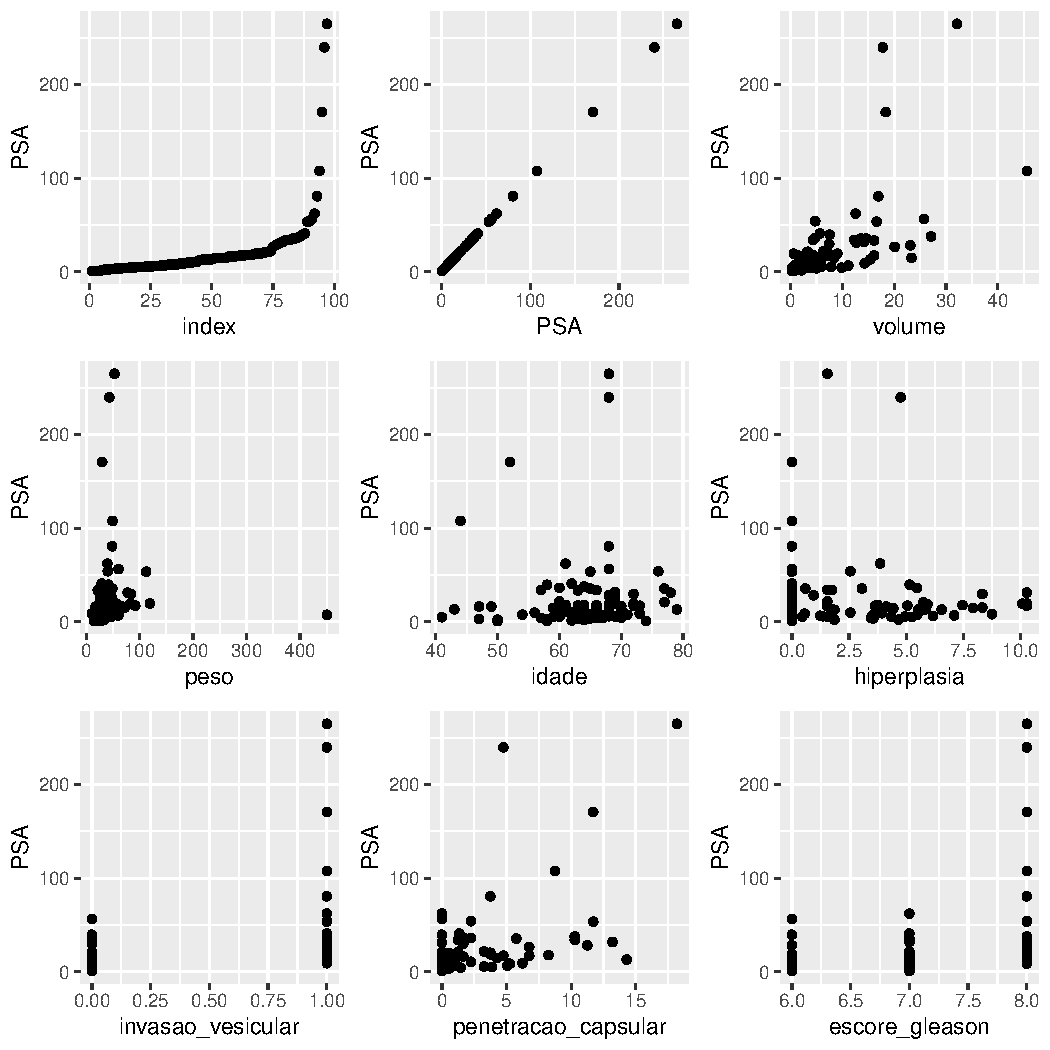
\includegraphics[width=\maxwidth]{figure/unnamed-chunk-6-1} 

\end{knitrout}
\vspace{-0.05cm}
Embora as correlações marginais entre o PSA  e as outras variáveis não seja elevado, estudos realizados anteriormente
constataram que o PSA varia quase linearmente com a idade e o o volume do câncer. \newpage
\begin{knitrout}
\definecolor{shadecolor}{rgb}{0.969, 0.969, 0.969}\color{fgcolor}
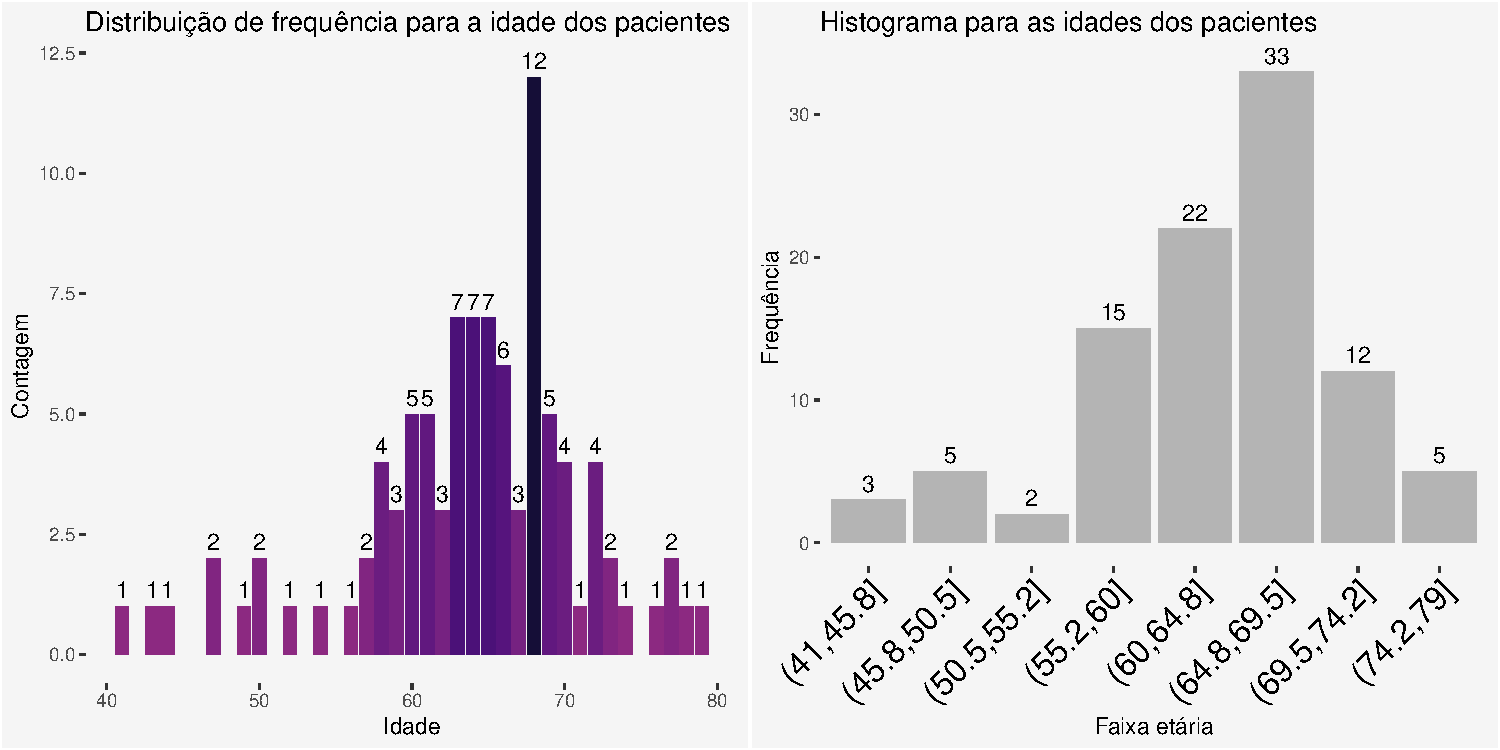
\includegraphics[width=\maxwidth]{figure/unnamed-chunk-7-1} 

\end{knitrout}
\begin{knitrout}
\definecolor{shadecolor}{rgb}{0.969, 0.969, 0.969}\color{fgcolor}
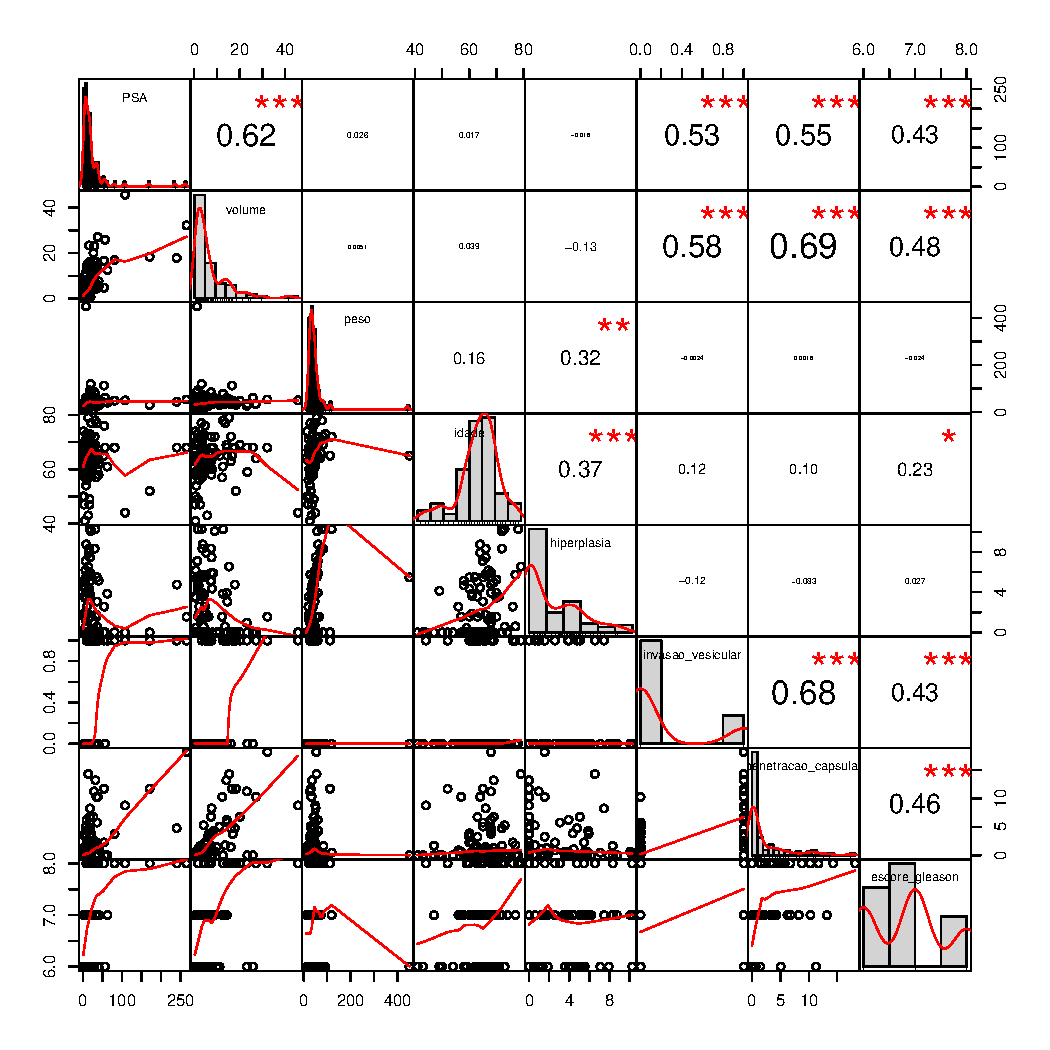
\includegraphics[width=\maxwidth]{figure/unnamed-chunk-8-1} 

\end{knitrout}
\newpage
No gráfico acima:
A distribuição empírica de cada variável é mostrada na diagona.
Abaixo da diagonal: Os diagramas de dispersão com uma curva ajustada.
Acima da diagonal estão os valores das correlaçõpes conjuntamente com seus níveis de significância:
Cada nível de significância está associado a uma certa quantidade de estrelas: i.e:$$\{(0, "***"),(0.001,"***"), (0.01,"**"), (0.05,"*"), (0.1,"."), (1,""))   \}$$

O boxplot abaixo mostra O nível de PSA para cada escore de Gleason.
Podemos observar que pacientes com Pontuação 8 no escore de Gleason possuem um PSA muito alto. De acordo com o instituto Oncoguia, se o nível do PSA é muito alto, a doença provavelmente está disseminada.
\\
\\

\begin{knitrout}
\definecolor{shadecolor}{rgb}{0.969, 0.969, 0.969}\color{fgcolor}
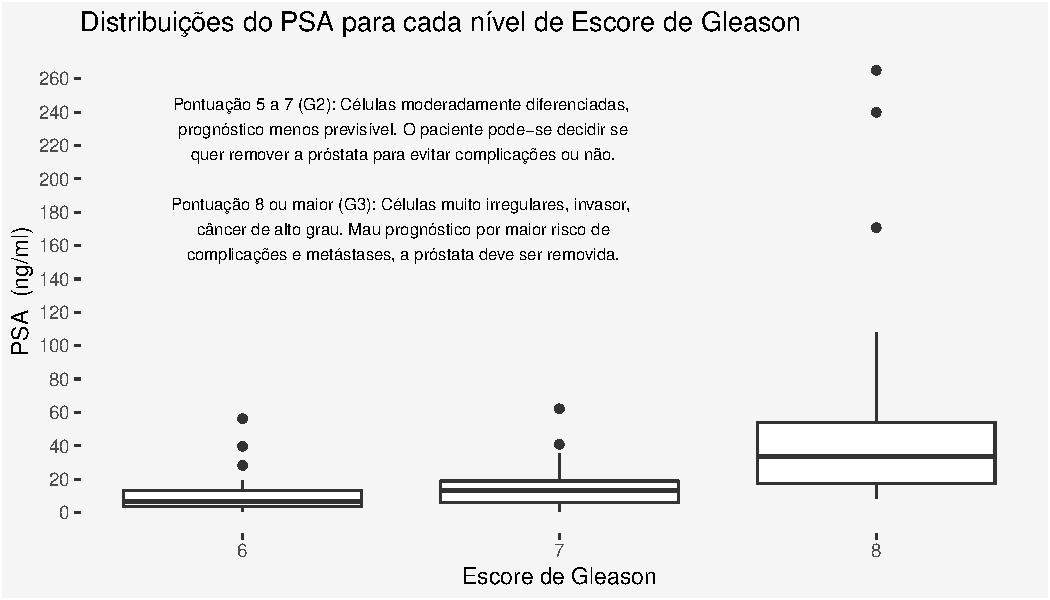
\includegraphics[width=\maxwidth]{figure/unnamed-chunk-9-1} 

\end{knitrout}
\begin{knitrout}
\definecolor{shadecolor}{rgb}{0.969, 0.969, 0.969}\color{fgcolor}
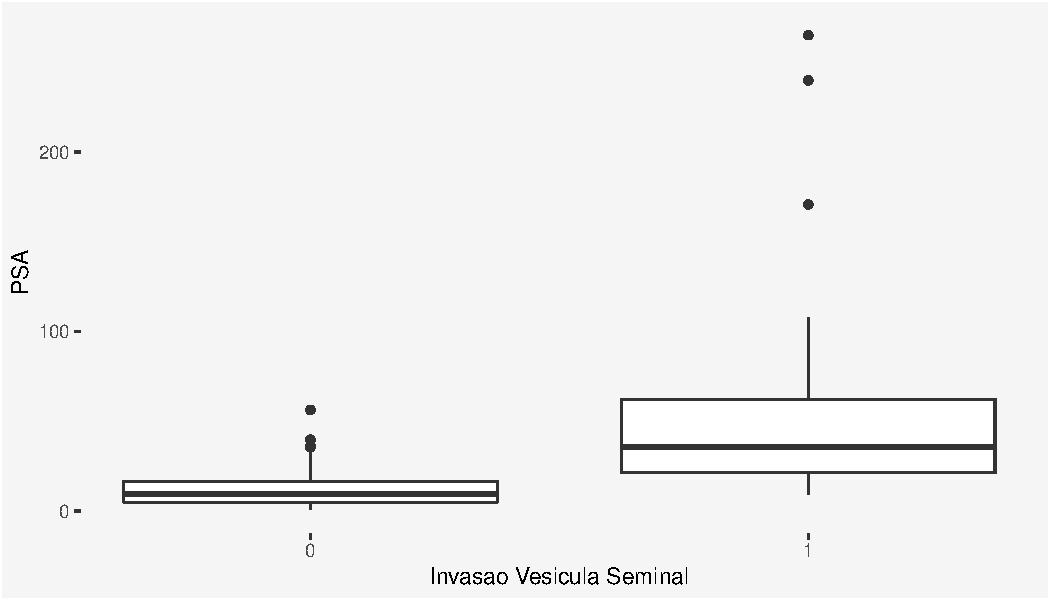
\includegraphics[width=\maxwidth]{figure/unnamed-chunk-10-1} 

\end{knitrout}
Dados os boxplots acima, podemos perceber que em pacientes que tiveram invasão vesicular, a mediana do nível de PSA é maior.

\begin{knitrout}
\definecolor{shadecolor}{rgb}{0.969, 0.969, 0.969}\color{fgcolor}\begin{table}

\caption{\label{tab:unnamed-chunk-11}Mediana de PSA entre pacientes com Invasão Vesícular (1) e sem (0).}
\centering
\begin{tabular}[t]{rr}
\toprule
invasao\_vesicular & Mediana\_PSA\\
\midrule
\rowcolor{gray!6}  0 & 9.356\\
1 & 35.517\\
\bottomrule
\end{tabular}
\end{table}


\end{knitrout}


\begin{knitrout}
\definecolor{shadecolor}{rgb}{0.969, 0.969, 0.969}\color{fgcolor}
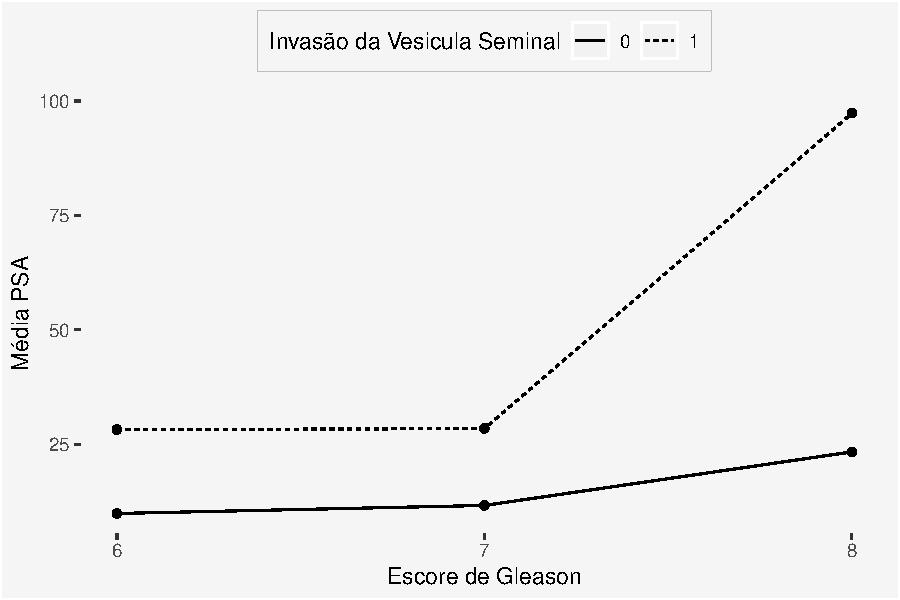
\includegraphics[width=\maxwidth]{figure/unnamed-chunk-12-1} 

\end{knitrout}

\section{Inferência e Modelagem}

Como não há indícios premiliminares de variáveis preditoras eficientes para a modelagem linear para o PSA, 
iremos ajustar, a princípio, um modelo completo, ou seja, com todas as variáveis: 

\begin{equation}
 V2 = \beta_0 V1 ... + \beta_9 V9 
\end{equation}
\begin{knitrout}
\definecolor{shadecolor}{rgb}{0.969, 0.969, 0.969}\color{fgcolor}\begin{table}

\caption{\label{tab:unnamed-chunk-13}Correlações entre todas as variáveis explicativas e seus respectivos valores p.}
\centering
\begin{tabular}[t]{llrr}
\toprule
row & column & cor & p\\
\midrule
\rowcolor{gray!6}  index & PSA & 0.603 & 0.0000000\\
index & volume & 0.621 & 0.0000000\\
\rowcolor{gray!6}  PSA & volume & 0.624 & 0.0000000\\
index & peso & 0.114 & 0.2673002\\
\rowcolor{gray!6}  PSA & peso & 0.026 & 0.7988241\\
\addlinespace
volume & peso & 0.005 & 0.9604030\\
\rowcolor{gray!6}  index & idade & 0.197 & 0.0536538\\
PSA & idade & 0.017 & 0.8672043\\
\rowcolor{gray!6}  volume & idade & 0.039 & 0.7038049\\
peso & idade & 0.164 & 0.1077533\\
\addlinespace
\rowcolor{gray!6}  index & hiperplasia & 0.165 & 0.1062806\\
PSA & hiperplasia & -0.016 & 0.8726613\\
\rowcolor{gray!6}  volume & hiperplasia & -0.133 & 0.1933412\\
peso & hiperplasia & 0.322 & 0.0013056\\
\rowcolor{gray!6}  idade & hiperplasia & 0.366 & 0.0002239\\
\addlinespace
index & invasao\_vesicular & 0.567 & 0.0000000\\
\rowcolor{gray!6}  PSA & invasao\_vesicular & 0.529 & 0.0000000\\
volume & invasao\_vesicular & 0.582 & 0.0000000\\
\rowcolor{gray!6}  peso & invasao\_vesicular & -0.002 & 0.9813051\\
idade & invasao\_vesicular & 0.118 & 0.2510649\\
\addlinespace
\rowcolor{gray!6}  hiperplasia & invasao\_vesicular & -0.120 & 0.2434580\\
index & penetracao\_capsular & 0.477 & 0.0000008\\
\rowcolor{gray!6}  PSA & penetracao\_capsular & 0.551 & 0.0000000\\
volume & penetracao\_capsular & 0.693 & 0.0000000\\
\rowcolor{gray!6}  peso & penetracao\_capsular & 0.002 & 0.9877539\\
\addlinespace
idade & penetracao\_capsular & 0.100 & 0.3319426\\
\rowcolor{gray!6}  hiperplasia & penetracao\_capsular & -0.083 & 0.4188958\\
invasao\_vesicular & penetracao\_capsular & 0.680 & 0.0000000\\
\rowcolor{gray!6}  index & escore\_gleason & 0.538 & 0.0000000\\
PSA & escore\_gleason & 0.430 & 0.0000113\\
\addlinespace
\rowcolor{gray!6}  volume & escore\_gleason & 0.481 & 0.0000006\\
peso & escore\_gleason & -0.024 & 0.8139337\\
\rowcolor{gray!6}  idade & escore\_gleason & 0.226 & 0.0261235\\
hiperplasia & escore\_gleason & 0.027 & 0.7942291\\
\rowcolor{gray!6}  invasao\_vesicular & escore\_gleason & 0.429 & 0.0000119\\
\addlinespace
penetracao\_capsular & escore\_gleason & 0.462 & 0.0000020\\
\bottomrule
\end{tabular}
\end{table}


\end{knitrout}

Os fatores de inflação de variância em conjunto com as correlações entre as variáveis explicativas
(VIF) não sao elevados e, portanto, nao temos indícios de multicolinearidade.
\begin{knitrout}
\definecolor{shadecolor}{rgb}{0.969, 0.969, 0.969}\color{fgcolor}\begin{table}

\caption{\label{tab:unnamed-chunk-14}Tolerância e VIF}
\centering
\begin{tabular}[t]{ccc}
\toprule
Variables & Tolerance & VIF\\
\midrule
\rowcolor{gray!6}  dados\$volume & 0.46 & 2.16\\
dados\$peso & 0.89 & 1.13\\
\rowcolor{gray!6}  dados\$idade & 0.81 & 1.24\\
dados\$hiperplasia & 0.76 & 1.31\\
\rowcolor{gray!6}  dados\$invasao\_vesicular & 0.50 & 2.01\\
\addlinespace
dados\$penetracao\_capsular & 0.40 & 2.52\\
\rowcolor{gray!6}  dados\$escore\_gleason & 0.69 & 1.46\\
\bottomrule
\end{tabular}
\end{table}

\begin{table}[H]
\centering
\begin{tabular}{rrrrr}
\toprule
Df & Sum Sq & Mean Sq & F value & Pr(>F)\\
\midrule
\rowcolor{gray!6}  1 & 62202.34 & 62202.34 & 64.03 & 0.00\\
1 & 84.66 & 84.66 & 0.09 & 0.77\\
\rowcolor{gray!6}  1 & 19.82 & 19.82 & 0.02 & 0.89\\
1 & 814.66 & 814.66 & 0.84 & 0.36\\
\rowcolor{gray!6}  1 & 7365.96 & 7365.96 & 7.58 & 0.01\\
\addlinespace
1 & 932.86 & 932.86 & 0.96 & 0.33\\
\rowcolor{gray!6}  1 & 1794.05 & 1794.05 & 1.85 & 0.18\\
89 & 86457.37 & 971.43 & NA & NA\\
\bottomrule
\end{tabular}
\end{table}


\end{knitrout}

\subsection{Selecção de Variáveis}

\begin{knitrout}
\definecolor{shadecolor}{rgb}{0.969, 0.969, 0.969}\color{fgcolor}\begin{kframe}
\begin{verbatim}
## 
## Call:
## lm(formula = PSA ~ volume + factor(invasao_vesicular), data = dados)
## 
## Residuals:
##     Min      1Q  Median      3Q     Max 
## -55.145  -7.535  -1.129   4.256 170.018 
## 
## Coefficients:
##                            Estimate Std. Error t value Pr(>|t|)    
## (Intercept)                   1.060      4.231   0.251   0.8027    
## volume                        2.477      0.495   5.003 2.62e-06 ***
## factor(invasao_vesicular)1   24.647      9.423   2.616   0.0104 *  
## ---
## Signif. codes:  0 '***' 0.001 '**' 0.01 '*' 0.05 '.' 0.1 ' ' 1
## 
## Residual standard error: 31.09 on 94 degrees of freedom
## Multiple R-squared:  0.431,	Adjusted R-squared:  0.4189 
## F-statistic:  35.6 on 2 and 94 DF,  p-value: 3.098e-12
\end{verbatim}
\end{kframe}
\end{knitrout}





\begin{knitrout}
\definecolor{shadecolor}{rgb}{0.969, 0.969, 0.969}\color{fgcolor}\begin{table}

\caption{\label{tab:unnamed-chunk-17}Tabela ANOVA para o modelo completo}
\centering
\begin{tabular}[t]{ccccc}
\toprule
Df & Sum Sq & Mean Sq & F value & Pr(>F)\\
\midrule
\rowcolor{gray!6}  1 & 62202.34 & 62202.34 & 64.03 & 0.00\\
1 & 84.66 & 84.66 & 0.09 & 0.77\\
\rowcolor{gray!6}  1 & 19.82 & 19.82 & 0.02 & 0.89\\
1 & 814.66 & 814.66 & 0.84 & 0.36\\
\rowcolor{gray!6}  1 & 7365.96 & 7365.96 & 7.58 & 0.01\\
\addlinespace
1 & 932.86 & 932.86 & 0.96 & 0.33\\
\rowcolor{gray!6}  1 & 1794.05 & 1794.05 & 1.85 & 0.18\\
89 & 86457.37 & 971.43 & NA & NA\\
\bottomrule
\end{tabular}
\end{table}

\begin{table}

\caption{\label{tab:unnamed-chunk-17}Tabela ANOVA para o modelo completo}
\centering
\begin{tabular}[t]{cccc}
\toprule
Estimate & Std..Error & t.value & Pr...t..\\
\midrule
\rowcolor{gray!6}  1.060368 & 4.23 & 0.25 & 0.8026785\\
2.476724 & 0.50 & 5.00 & 0.0000026\\
\rowcolor{gray!6}  24.647065 & 9.42 & 2.62 & 0.0103769\\
\bottomrule
\end{tabular}
\end{table}

\begin{table}

\caption{\label{tab:unnamed-chunk-17}Tabela ANOVA para o modelo reduzido}
\centering
\begin{tabular}[t]{ccccc}
\toprule
Df & Sum Sq & Mean Sq & F value & Pr(>F)\\
\midrule
\rowcolor{gray!6}  1 & 62202.34 & 62202.34 & 64.354257 & 0.0000000\\
1 & 6612.59 & 6612.59 & 6.841357 & 0.0103769\\
\rowcolor{gray!6}  94 & 90856.77 & 966.56 & NA & NA\\
\bottomrule
\end{tabular}
\end{table}


\end{knitrout}
Embora a idade seja um fator relevante para explicar o PSA, nossos dados não capturaram bem essa característica. Sendo assim iremos utilizar um modelo reduzido para explicar a variabilidade do PSA.
\begin{equation}
  E[PSA_i] = \beta_0 volume\_cancer+ \beta_1 invasao\_vesicular
\end{equation}
\section{Diagnóstico }
Nesta sessão iremos realizar a anáçise de diagnóstico. A Análise de diagnóstico é importante para verificar se o modelo proposto, quando ajustado aos dados, satisfaz as suposições do modelo linear normal.
Por mínima que seja a fulga dessas suposiçõpes, as consequências podem ser catastróficas, pois podem tornar o modelo viesado, e as estimativas não serão mais eficientes no sentido de que suas variâncias não serão as menores na classe dos estimadores BLUE.

\begin{knitrout}
\definecolor{shadecolor}{rgb}{0.969, 0.969, 0.969}\color{fgcolor}
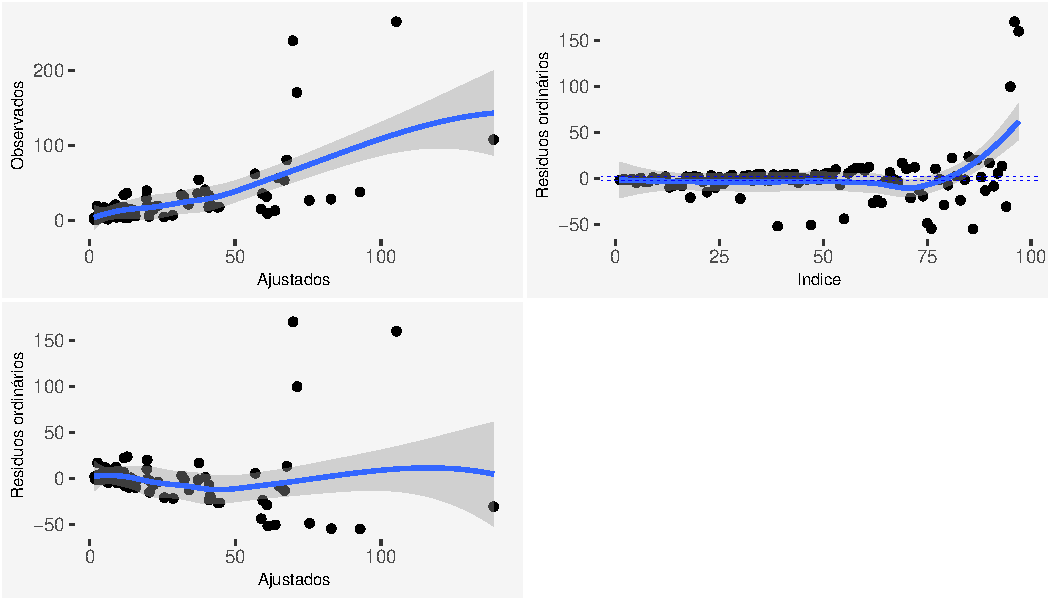
\includegraphics[width=\maxwidth]{figure/unnamed-chunk-18-1} 

\end{knitrout}


\begin{knitrout}
\definecolor{shadecolor}{rgb}{0.969, 0.969, 0.969}\color{fgcolor}
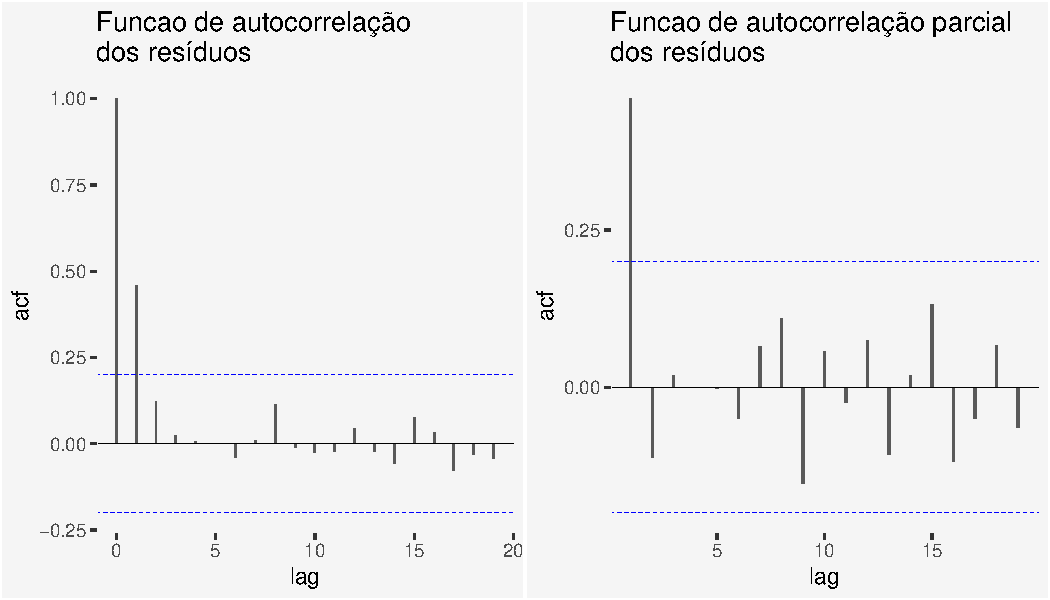
\includegraphics[width=\maxwidth]{figure/unnamed-chunk-19-1} 

\end{knitrout}

Podemos observar que a FAC para os resíduos indicam um decaimento exponencial, com duas barras ultrapassando o limite. Sugerindo, assim, que exista autocorrelação nos resíduos e que essa autocorrelação pode ser modelada por um AR(2). 
Já, a FACP sugerem um modelo MA(1). Sendo assim, os residuos podem ser modelados por um processo ARMA(2,1).


\begin{knitrout}
\definecolor{shadecolor}{rgb}{0.969, 0.969, 0.969}\color{fgcolor}
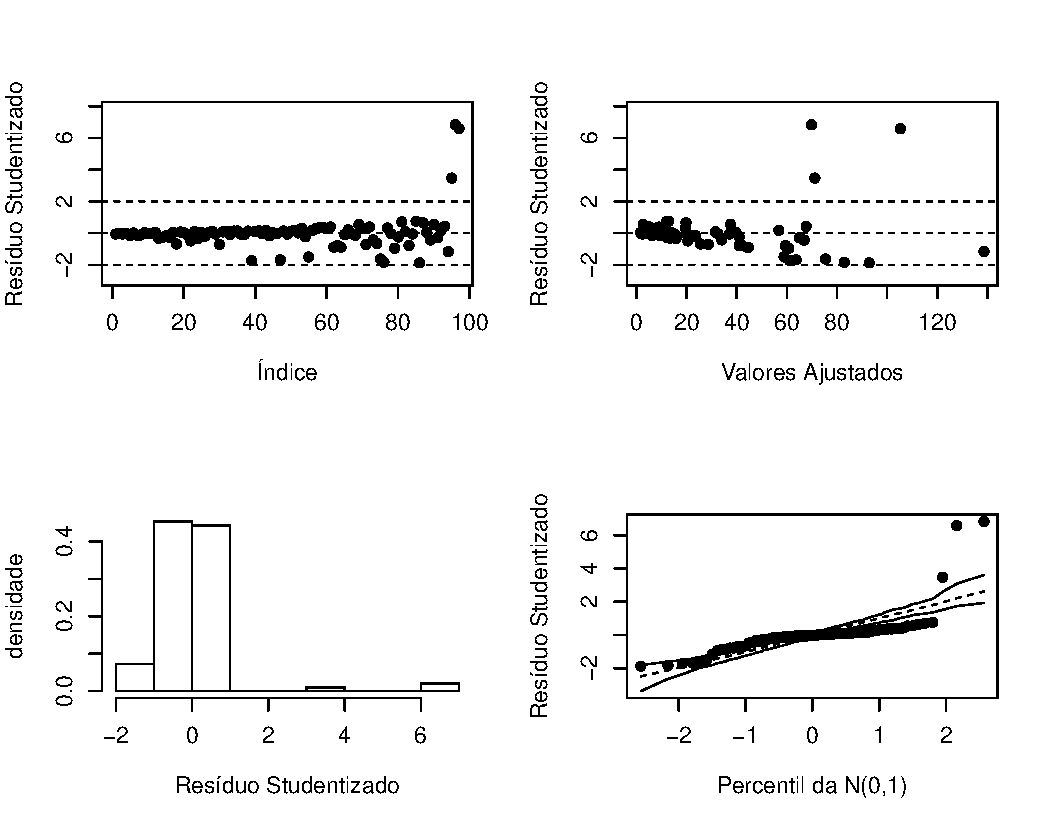
\includegraphics[width=\maxwidth]{figure/unnamed-chunk-20-1} 

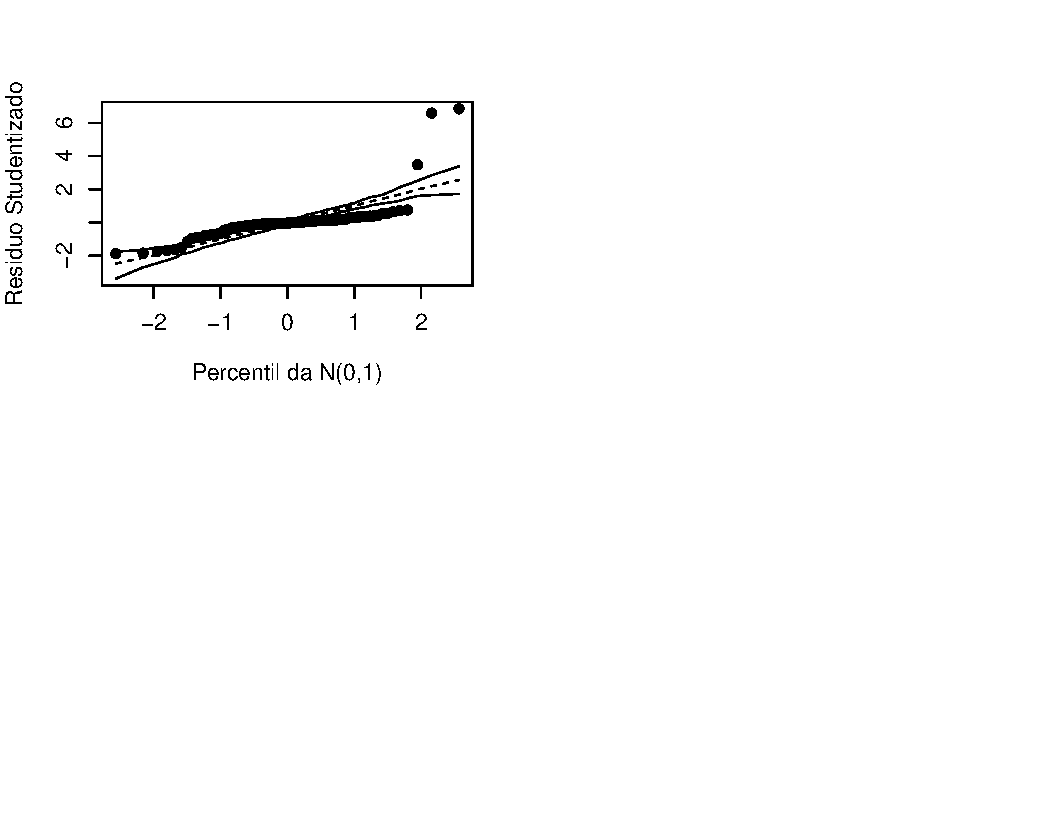
\includegraphics[width=\maxwidth]{figure/unnamed-chunk-20-2} 

\end{knitrout}

\section{Conclusões}
Durante o estudo foram obtidos diversos indícios de que um modelo de regressão Linear possa não ser adequado para modelar esse tipo de dados, tendo em vista que os graficos de diagnostico corroboram com essa afirmação, podemos rejeitar e propor outros modelos da mais generalizados que possam se adequar bem aos dados sem fugir das suposições.

Não obtante, um possivel modelo inicial que resolvi escolher é dado por:

  \[
    E(PSA|Volume, Invasao)=\begin{cases}
                1.060+2.477 Volume+24.647, \ \text{se houve invasão da vesicula seminal}\\
                1.060+2.477 Volume,  \ \text{Caso Contrário}
    \end{cases}
  \]
  
Ou seja, o fato de haver invasão da vesicula semina causa uma variação no intercepto de 23,25 \% no nível de PSA do paciente quando o volume do cancer é o mínimo possivel.

\newpage
\begin{thebibliography}{9}
\bibitem{SEARLE}
  SEARLE, Shayli R.
  \textit{\textbf{Linear Models}},
  2nd edition,
  Hoboken, N.J.: Wiley Interscience,
  2003.

\bibitem{japan}
  AMIT GUPTA, CORINNE ARAGAKI, MOMOKAZU GOTOH, NAOYA MASUMORI, SHINICHI OHSHIMA, TAIJI TSUKAMOTO, CLAUS G. ROEHRBORN.
  \textit{\textbf{RELATIONSHIP BETWEEN PROSTATE SPECIFIC ANTIGEN AND INDEXES OF PROSTATE VOLUME IN JAPANESE MEN}},
The Journal of Urology,
Volume 173, Issue 2,
2005,
Pages 503-506,
ISSN 0022-5347
\end{thebibliography}
\newpage
\end{document}
